\documentclass{article}

% If you're new to LaTeX, here's some short tutorials:
% https://www.overleaf.com/learn/latex/Learn_LaTeX_in_30_minutes
% https://en.wikibooks.org/wiki/LaTeX/Basics

% Formatting
\usepackage[utf8]{inputenc}
\usepackage[margin=1in]{geometry}
\usepackage[titletoc,title]{appendix}

% Math
% https://www.overleaf.com/learn/latex/Mathematical_expressions
% https://en.wikibooks.org/wiki/LaTeX/Mathematics
\usepackage{amsmath,amsfonts,amssymb,mathtools}

% Images
% https://www.overleaf.com/learn/latex/Inserting_Images
% https://en.wikibooks.org/wiki/LaTeX/Floats,_Figures_and_Captions
\usepackage{graphicx,float}

% Tables
% https://www.overleaf.com/learn/latex/Tables
% https://en.wikibooks.org/wiki/LaTeX/Tables

% Algorithms
% https://www.overleaf.com/learn/latex/algorithms
% https://en.wikibooks.org/wiki/LaTeX/Algorithms
\usepackage[ruled,vlined]{algorithm2e}
\usepackage{algorithmic}

% Code syntax highlighting
% https://www.overleaf.com/learn/latex/Code_Highlighting_with_minted
\usepackage{minted}
\usemintedstyle{borland}

% References
% https://www.overleaf.com/learn/latex/Bibliography_management_in_LaTeX
% https://en.wikibooks.org/wiki/LaTeX/Bibliography_Management
\usepackage{biblatex}
\addbibresource{references.bib}

% Title content
\title{CMPT 354 Project Proposal}
\author{Group 59}
\date{February 22, 2021}

\begin{document}

\maketitle

% Abstract
\begin{abstract}
    Data of past precipitation and water usage in Greater Vancouver can provide insight into potential future droughts where water restrictions may be necessary. By carefully analyzing past patterns, governments and people can know ahead of time when to expect constraints on water usage. Machine learning algorithms can be leveraged to provide accurate predictions, allowing for early action and increased public acceptance.
\end{abstract}

\section{Domain}
Water conservation has been an ongoing concern throughout the world for over half a century. While Canada has a generous amount of water supply, there is still a responsibility to hold with keeping that resource healthy. Using machine learning, citizens of Greater Vancouver can support this by learning when and how to modify their water usage to avoid potential droughts.

\section{Application Specifications}
Our project has two major aspects to it, both contributing to water conservation and transparency. Water source and water consumption data may be organized in a relational database to allow for simple information extraction via queries. In addition to the relational database aspect, the project will include a machine learning model trained to provide likely prediction of water fluctuations.

Among possible queries is the possibility to obtain water usage information from an array of water users. Water users come in the form of households, businesses, or government-run facilities. Each disjoint water user entity may be queried for information regarding how much water was consumed over a given amount of time. Much can be derived from this information, such as average, maximum, and minimum water usage over time. The database includes an additional entity of water sources. Water sources belong to a region and have attributes such as water capacity and water levels over time.

With the data strung together in the relational database, a machine learning model can accomplish what is not possible by a query language. Our project will implement a machine-learning algorithm to find patterns in the past and suggest trends in the future.

Our project will serve as a medium to access both water consumption and water level information from regions, as well as provide an insight into future water usage.


\section{Application Stack}
Our project will be implemented as a web app accessible online. To accomplish this, our team will utilize the Flask micro web framework written in Python. Flask will provide a simplistic, yet powerful means by which to implement the project. The abstractions provided by Python will allow our team to adopt agile practices without the baggage inevitable with more syntactically verbose languages.

To represent the Database Management System (DBMS) will be MySQL. MySQL is an industry-leading DBMS known for reliability and quick processing.

\section{EER Diagram}

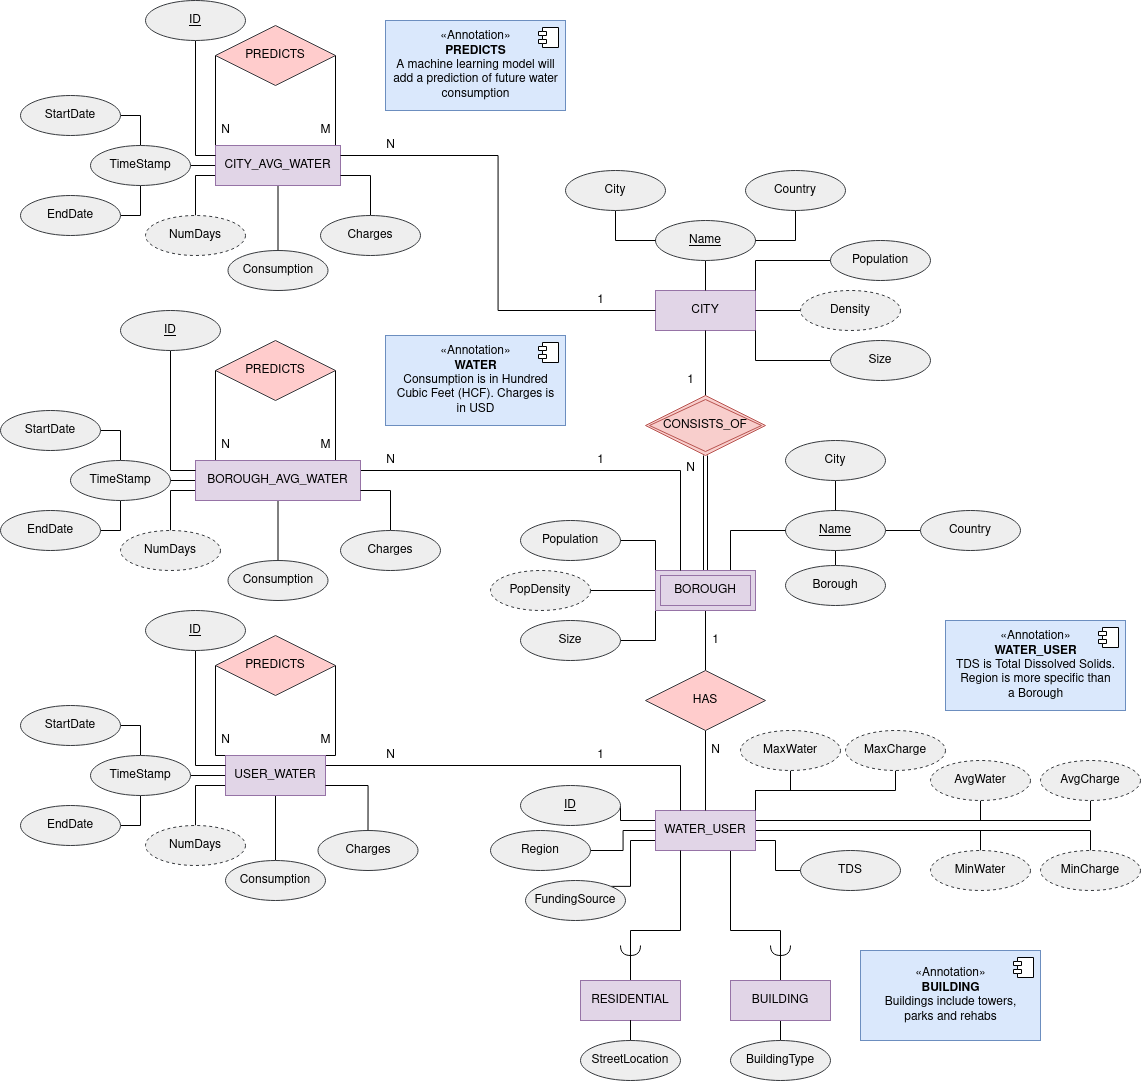
\includegraphics[width=\linewidth]{UML_Diagram.png}
\centering {
Figure 1: EER diagram representing the water conservation relational database
}
% begin{figure}[tb] % t = top, b = bottom, etc.
% \begin{figure}[t]
%     \centering
%     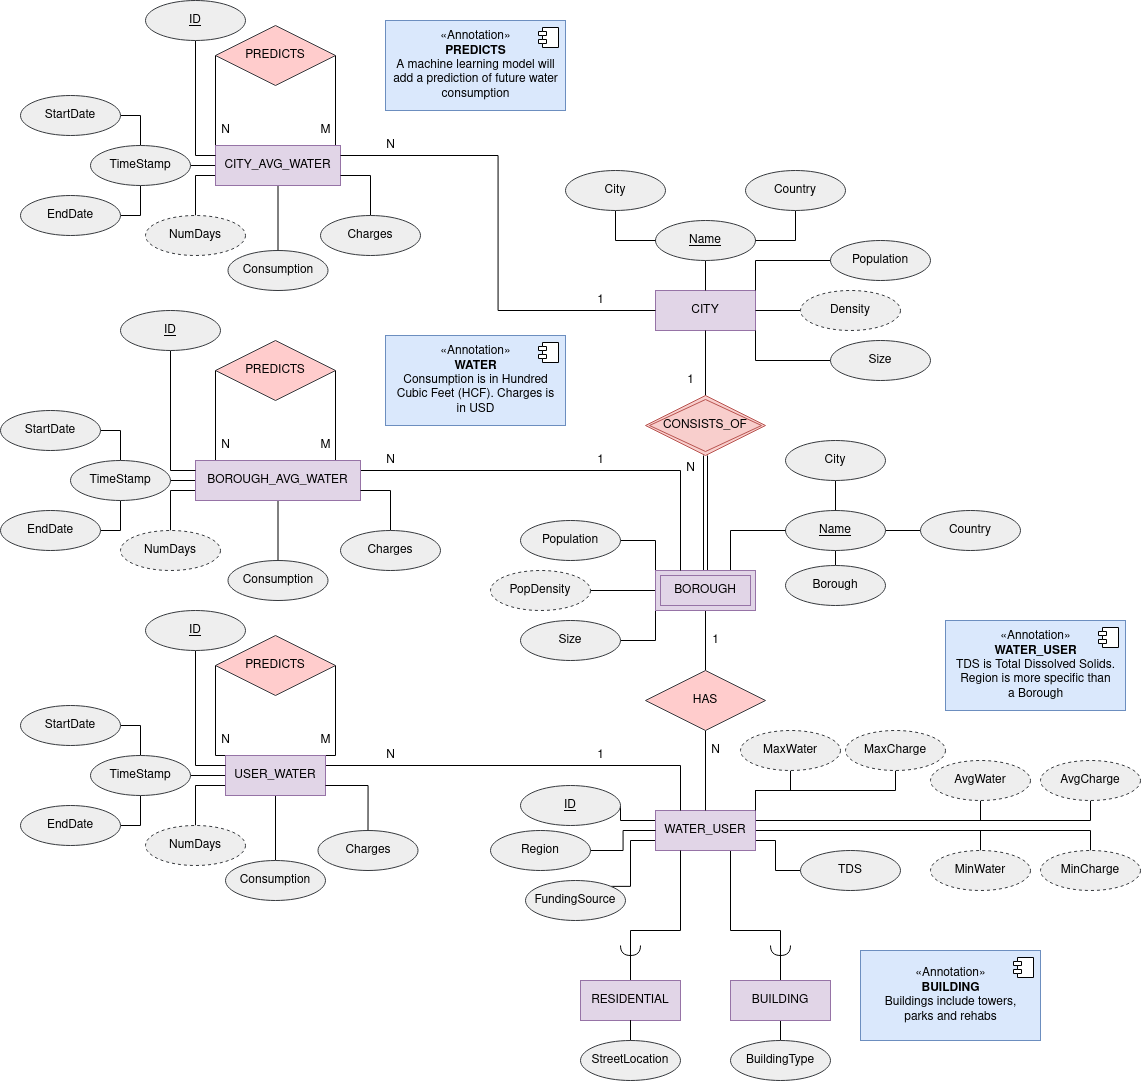
\includegraphics[width=\linewidth]{UML_Diagram.png}
%     \caption{EER diagram representing water conservation relational database}
%     \label{fig:dubs}
% \end{figure}


\end{document}
